%! Author = gramic
%! Date = 15.03.24

% Preamble
\begin{flushleft}
    \subsubsection{StackGres - Citus}
    \paragraph{Architektur}
    Für das Benchmarking wurde ein minimales setting ausgewählt.\\
    Ein Coordinator und einen Shard-Node mit einem Leader- und Replica-Pod.\\
    \begin{figure}[H]
        \centering
        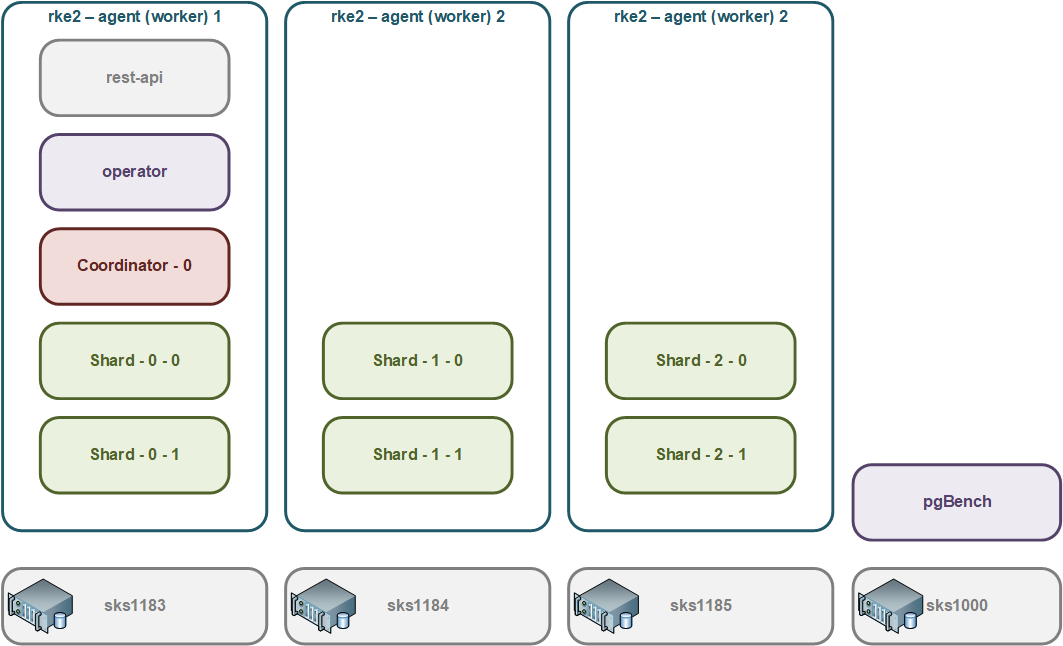
\includegraphics[width=0.8\linewidth]{source/implementation/evaluation/postgresql_ha_solutions/stackgres/stackgres-citus-evaluation-architecture}
        \caption{Stackgres - Citus - Evaluationsarchitektur Benchmarking}
        \label{fig:stackgres-citus-evaluation-architecture}
    \end{figure}
    Für die Self Healing Tests wurde eine umfangreichere Architektur vorgenommen.\\
    Es stellte sich heraus, dass man relativ leicht die beim \hyperref[subpar:citus_sharding]{Citus Sharding} beschriebene Lösung zum Replizieren leicht umzusetzen ist:
    \begin{figure}[H]
        \centering
        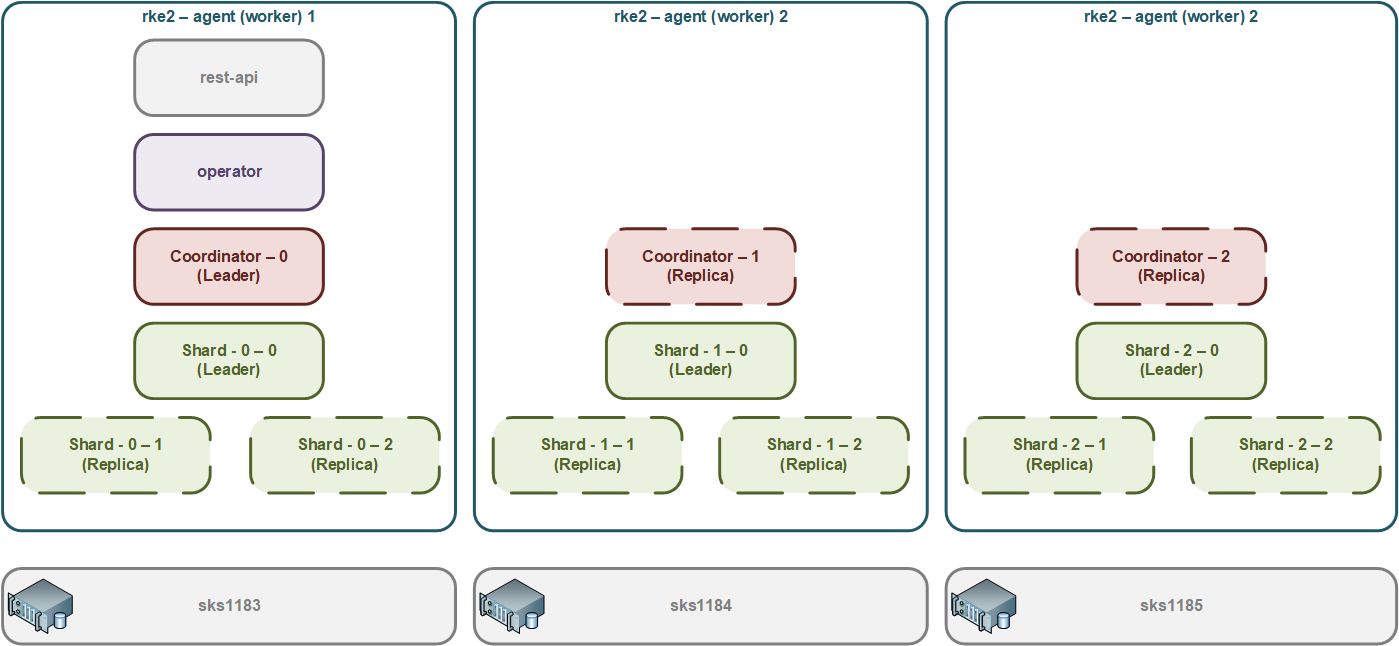
\includegraphics[width=0.8\linewidth]{source/implementation/evaluation/postgresql_ha_solutions/stackgres/stackgres_citus_architecture_self_healing_test}
        \caption{Stackgres - Citus - Evaluationsarchitektur Self Healing Tests}
        \label{fig:stackgres_citus_architecture_self_healing_test}
    \end{figure}
\end{flushleft}
\begin{flushleft}
    \paragraph{Ressourcenhunger}
    Aus den Architekturschemen ist bereits ersichtlich, dass StackGres sehr viele Pods erstellt.\\
    StackGres erzeugt mindestens einen Operator- und einen REST-API-Pod, der aber auch für das GUI verwendet wird.\\
    Nun kommt der Coordinator-Pod hinzu und je nach Auswahl pro Node ein Shard-Pod wobei es mindestens eine Instanz braucht.\\
    Will heissen, im Worst-Case sind auf einem Node mindestens 4 Pods, auf dem Server kann aber auch noch der k8s-server (control-plane) stehen.\\
    Pro Pod muss mindestens eine CPU gesetzt werden, auch der k8s-Server benötigt mindestens eine CPU, heisst das pro Server mit Minimal setting 5 CPUs benötigt werden:
    \begin{figure}[H]
        \centering
        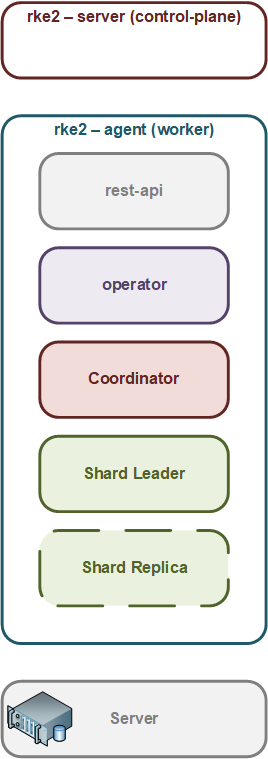
\includegraphics[width=0.1\linewidth]{source/implementation/evaluation/postgresql_ha_solutions/stackgres/stackgres_citus_architecture_resource_stack}
        \caption{Stackgres - Citus - Resourcen - Stack}
        \label{fig:stackgres_citus_architecture_resource_stack}
    \end{figure}
    Auch Memory und Storage muss eingerechnet werden, besonders wenn pro Shard noch mehrere Instanzen deployt werden sollen.
    Dazu kommt noch eine weitere eigenheit von StackGres.
\end{flushleft}
\begin{flushleft}
    Dazu kommt noch eine weitere eigenheit von StackGres.\\
    Pro Datenbank wird Standardmässig ein Cluster erstellt mit jeweils mindestens einem Coordinator und dem ganzen Stack der daran hängt:
    \begin{figure}[H]
        \centering
        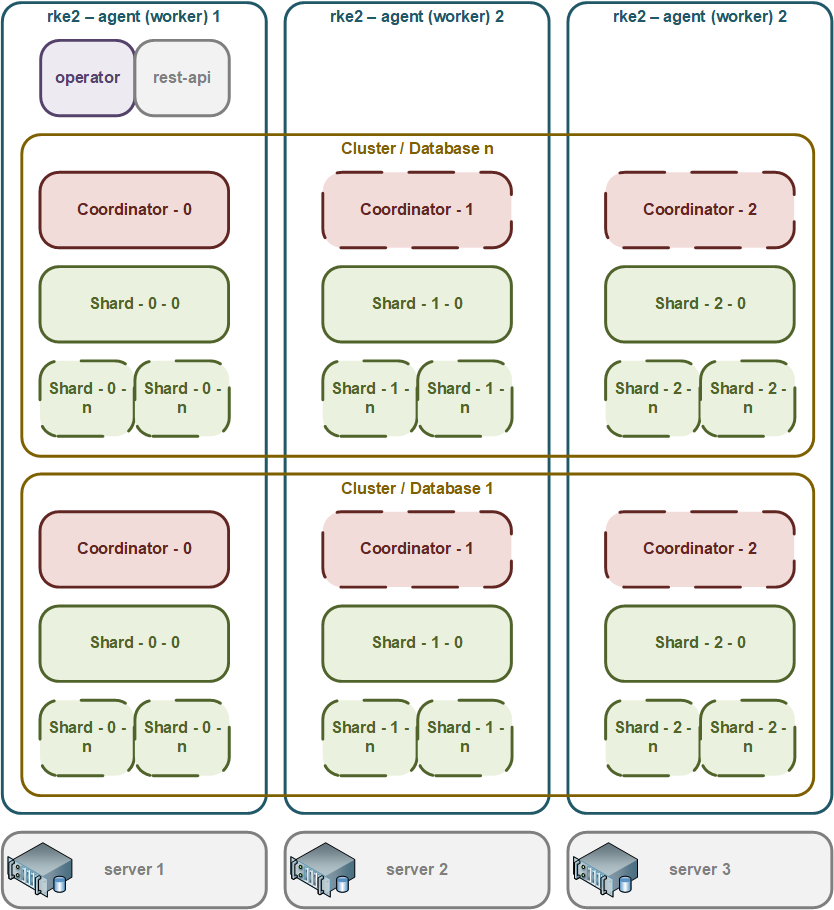
\includegraphics[width=0.1\linewidth]{source/implementation/evaluation/postgresql_ha_solutions/stackgres/stackgres_citus_architecture_clustering}
        \caption{Stackgres - Citus - Datenbank - Cluster}
        \label{fig:stackgres_citus_architecture_clustering}
    \end{figure}
    Entsprechend steigt der Ressourcenbedarf zusätzlich.
\end{flushleft}
\begin{flushleft}
    \paragraph{Installation}
    OnGres bietet für StackGres ein \gls{helm}-Chart, welches über ein eigenes \texttt{values.yaml}-Manifest oder direkt aus dem Repository mittels Parametern deployet werden kann.\\
    Beim KSGR wurde das \gls{helm}-Chart heruntergeladen und entsprechend ein eigenes Manifest geschrieben.
\end{flushleft}
\begin{flushleft}
    StackGres bietet von Haus aus an, einen Sharded Cluster mit Citus zu installieren.\\
    Dabei muss allerdings das StackGres Extension Repository erreichbar sein, welches mit \texttt{https} erreichbar sein muss.
\end{flushleft}
\begin{flushleft}
    Hier wird es nun knifflig, sobald Proxys im Spiel sind.\\
    Selbst wenn die Proxy-Settings auf dem Host und im \gls{rke2} (\texttt{CONTAINERD\_HTTPS\_PROXY} / \texttt{CONTAINERD\_HTTP\_PROXY} / \texttt{CONTAINERD\_NO\_PROXY}) gesetzt sind,\\
    ist dies keine Garantie das mittels \texttt{https} aus dem Pod heraus kommuniziert werden kann, selbst wenn es mit \texttt{curl} möglich ist.\\
    Damit dies möglich ist, müssen die Proxy-Zertifikate auf den Host installiert werden.\\
    Alternativ kann die Kommunikation über \texttt{http} erzwungen werden.\\
    StackGres bietet diese möglichkeit und da es sich um eine Evaluationsumgebung handelt, wurde dieser Weg gewählt.\\
    Zum einen muss der Proxy nach der \texttt{proxyUrl} eingegeben werden, danach müssen die Parameter \texttt{skipHostnameVerification:true} und \texttt{setHttpScheme:true} gesetzt werden.\\
    Die Proxy-URL muss dabei wie folgt aufgebaut werden:
\lstset{style=gra_codestyle}
\begin{lstlisting}[language=yaml, caption=StackGres - values.yaml - Extension proxyUrl,captionpos=b,label={lst:stackgres_extension_proxyurl},breaklines=true]
<proxy scheme>%3A%2F%2F<proxy host>%3A<proxy port>
\end{lstlisting}
    Proxy Schema meint dabei \texttt{http} oder \texttt{https}
    Für den KSGR-Proxy sieht der gesamte String entsprechend so aus:
\lstset{style=gra_codestyle}
\begin{lstlisting}[language=yaml, caption=StackGres - values.yaml - Extension Proxy,captionpos=b,label={lst:stackgres_extension_proxy},breaklines=true]
extensions:
  repositoryUrls:
  - https://extensions.stackgres.io/postgres/repository?proxyUrl=http%3A%2F%2Fsproxy.sivc.first-it.ch%3A8080?skipHostnameVerification:true&setHttpScheme:true
\end{lstlisting}
%\end{flushleft}
%\begin{flushleft}
    Die Ursachenforschung hat viel Zeit in Anspruch genommen.\\
    Es sind nebst dem Versuch, eine Freigabe via Pod-Affinität zu lösen, drei Tage verstrichen bis StackGres die Extensions ausführen konnte.
\end{flushleft}
\begin{flushleft}
    Anders als bei YugabyteDB, kann man das Web-GUI nicht mittels eines Load Balancer Exposing nach aussen präsentieren, auch wenn eine Cluster-IP gesetzt werden kann.\\
    Soll das Web-GUI und die REST-API permanent von aussen verfügbar sein, muss auf dem rest-api Pod ein permanentes Forwarding implementiert werden.\\
    Umsetzen lässt sich dies mittels der entsprechenden Keys im \texttt{values.yaml} oder den Parametern beim Deploy.
\end{flushleft}
\begin{flushleft}
    \paragraph{Cluster Deployment}
    Mit der Installation von StackGres steht noch keine Datenbank, es steht nur der Operator- und REST-API Pod.\\
    Dabei muss unterschieden werden, ob eine normale Patroni-Instanz deployt werden soll oder eine Sharded-Instanz (mit Citus).\\
    Dazu braucht es vorgängig folgende Ressourcen, die deployt werden müssen:\\
    \begin{description}
        \item \textbf{StorageClass}\hfill \\Die StorageClass für den Cluster.\\Je nachdem empfiehlt es sich, für den Coordinator eine eigene StorageClass zu erzeugen.
        \item \textbf{SGInstanceProfile}\hfill \\Das Instanz-Profil definiert, wie viel CPU und Memory der Pod erhält.\\Die konfigurationsmöglichkeiten gehen so tief,\\das innerhalb von Pods auch Containern Ressourcen zugewiesen werden können.\\ Empfehlenswert ist, Coordinator und Worker zu trennen.\\Ohne ein separates Instanz-Profil wird ein Standardprofil mit einer CPU und einem GiB Memory allokiert.
        \item \textbf{SGPostgresConfig}\hfill \\PostgreSQL-Spezifische Einstellungen können hierüber konfiguriert werden.\\Wie das Instanz-Profil auch, ist dies nicht zwingend, allerdings wird dann eine PostgreSQL-DB mit minimalem Setting deployt.
        \item \textbf{SGShardedCluster}\hfill \\Mit diesem Manifest wird der Cluster oder Sharded Cluster deployt.\\Eigene Ressourcen wie Instanz-Profile müssen entsprechend deklariert werden.
    \end{description}
\end{flushleft}
\begin{flushleft}
    Beim \texttt{SGShardedCluster}-Manifest gilt es einige Punkte zu beachten.\\
    Wird beim Coordinator mehr als eine Instanz angegeben, so wird der Coordinator mittels Patroni in einem Replica-Cluster betrieben.\\Dies hat den Vorteil, dass der Unterbruch bei einem Node Failure kleiner ist.
\end{flushleft}
\begin{flushleft}
    Bei den \texttt{shards} gibt es allerdings zwei Parameter die entscheidend sind.\\Zum einen \texttt{clusters}, die entsprechend die Anzahl an Shard-Pods erzeugen.\\
    Es müssen dann aber auch die Anzahl Instanzen beim Parameter \texttt{instancesPerCluster} gesetzt werden.\\Bei nur einer Instanz wird keine Replikation auf die Nodes erzeugt, bei mehr als einer Instanz wird auf die Nodes verteilt.\\
    Bei drei Nodes und drei Instanzen wird entsprechend auf alle Nodes repliziert, bei zwei Instanzen nur auf zwei von drei Nodes.
\end{flushleft}
\begin{flushleft}
    Damit die PostgreSQL-DB, hier in Form vom Service \texttt{postgresServices}, von ausserhalb erreichbar ist,\\muss die IP-Adresse von \Gls{MetalLB} gebunden werden.\\
    Zentral ist dabei die Annotation für den Primary-Service:
\lstset{style=gra_codestyle}
\begin{lstlisting}[language=yaml, caption=StackGres-Citus - LoadBalancer -Annotation,captionpos=b,label={lst:stackgres-citus-loadbalancer-annotation},breaklines=true]
  postgresServices:
    coordinator:
      primary:
        type: LoadBalancer
      any:
        type: LoadBalancer
    shards:
      primaries:
        type: LoadBalancer
  metadata:
    annotations:
      primaryService:
        metallb.universe.tf/loadBalancerIPs: 10.0.20.106
      replicasService:
        metallb.universe.tf/loadBalancerIPs: 10.0.20.153
        externalTrafficPolicy: "Cluster"
\end{lstlisting}
\end{flushleft}
\begin{flushleft}
    Das erzeugen von Persistent Volume Claims für Coordinator- und Shard-Pods wird wie folgt deklariert (hier nur mit der StorageClass \texttt{stackgres-storage}):
\lstset{style=gra_codestyle}
\begin{lstlisting}[language=yaml, caption=StackGres-Citus - StorageClass -PVC Binding,captionpos=b,label={lst:stackgres-citus-storageclass-pvc},breaklines=true]
...
  coordinator:
    ...
    pods:
      persistentVolume:
        size: '<Grösse>Gi'
        storageClass: "stackgres-storage"
...
  shards:
    ...
    pods:
      persistentVolume:
        size: 'GrösseGi'
        storageClass: "stackgres-storage"
\end{lstlisting}
\end{flushleft}
\begin{flushleft}
    Die Instanz-Profile lassen sich wie folgt zuweisen:
\lstset{style=gra_codestyle}
\begin{lstlisting}[language=yaml, caption=StackGres-Citus - Instanz-Profile, captionpos=b,label={lst:stackgres-citus-sginstanceprofile},breaklines=true]
  ...
  coordinator:
    instances: 1
    ...
    sgInstanceProfile: "<Instanz-Profil Coordinator>"
  ...
  shards:
    ...
    sgInstanceProfile: "<Instanz-Profil Shard>"
\end{lstlisting}
\end{flushleft}
\begin{flushleft}
    Beim Benchmarking kam es zu einem sehr unschönen Fehler.\\
    PgBounder verlor die Verbindung.\\
    Nach einer kurzen Suche, zeigte sich das es wohl einen Bug bei grösseren Workloads gibt, zumindest ist dies meine Interpretation.\\
    Die Lösung bei einigen schien zu sein, dass das Pooling abgeschaltet wird\cite{JU2PRK9L}.\\
    Für das Benchmarking wurde dies dann auch umgesetzt.\\
    Dies wird folgendermassen gemacht:
\lstset{style=gra_codestyle}
\begin{lstlisting}[language=yaml, caption=StackGres-Citus - StorageClass -PVC Binding,captionpos=b,label={lst:stackgres-citus-disable-pooler},breaklines=true]
...
  coordinator:
    pods:
      ...
      disableConnectionPooling: true
...
\end{lstlisting}
    Bei einem produktiven System müsste dieser Bug aber gefixt werden.
\end{flushleft}
\begin{flushleft}
    Bei einem Drei-Node Environment wie es für die Evaluation verwendet wird,\\kommt es zu einem Konflikt, wenn drei Shard-Pods erzeugt werden.\\
    In diesem Fall muss ein Testing- oder Development-Profil gesetzt werden.\\
    Alternativ können Pod Anti-Affinities oder Pod Affinities gesetzt werden, was sich aber als schwieriges unterfangen auszeichnete da Ongres dies nicht wirklich Dokumentiert hat.\\
    Daher wurde immer ein Testing-Profil gesetzt:
\lstset{style=gra_codestyle}
\begin{lstlisting}[language=yaml, caption=StackGres-Citus - Cluster Profil,captionpos=b,label={lst:stackgres-citus-cluster-profile},breaklines=true]
apiVersion: stackgres.io/v1alpha1
kind: SGShardedCluster
metadata:
  name: <cluster / db name>
  namespace: <cluster namespace>
spec:
  ...
  profile: "testing"
\end{lstlisting}
\end{flushleft}
\begin{flushleft}
    Es gäbe zwar die Möglichkeit, Passwörter via Manifest zu setzen, aber dies funktioniert nicht für postgres- und replicator sowie backup.\\
    Laut der StackGres-Dokumentation müssen z.B. die Passwörter vom \texttt{postgres}-User im Nachgang via SQL geändert werden.\\
    Während der Evaluation wurde darauf verzichtet und das generische Passwort aus dem Cluster geholt.
\end{flushleft}
\begin{flushleft}
    Die vollständige Dokumentation der Evaluationsinstallation ist im \hyperref[subsec:evaluation_installation_stackgres]{Anhang - Installation StackGres - Citus} zu finden.
\end{flushleft}